% Рисунок из тетради: 1/x на (0,1) — пример функции из L^1_loc((0,1)).
\begin{figure}[htbp]
\centering
\begin{tikzpicture}
\begin{axis}[
  width=8cm, height=5cm,
  axis lines=middle,
  xmin=-0.1, xmax=1.35,
  ymin=-0.9, ymax=7.5,
  xtick={1}, xticklabels={$1$},
  ytick=\empty,
  samples=120, clip=false,
]
  \addplot[very thick, blue!60!black, domain=0.14:1.3] {1/x};
  \draw[dashed, gray] (axis cs:0,0) -- (axis cs:0,7.2);
  \node[blue!60!black, anchor=west] at (axis cs:0.42,5.2) {$\tfrac1x$};
  \node[anchor=north] at (axis cs:0,-0.1) {$0$};

  % отрезок [a,b], строго внутри (0,1)
  \draw[very thick, red!70!black] (axis cs:0.3,-0.45) -- (axis cs:0.85,-0.45);
  \draw[very thick, red!70!black] (axis cs:0.3,-0.3) -- (axis cs:0.3,-0.6);
  \draw[very thick, red!70!black] (axis cs:0.85,-0.3) -- (axis cs:0.85,-0.6);
  \node[red!70!black, anchor=north, font=\footnotesize] at (axis cs:0.575,-0.62)
       {$\Omega' \Subset (0,1)$};
\end{axis}
\end{tikzpicture}
\caption{$\tfrac1x \in L^1_{\mathrm{loc}}((0,1))$: на любом отрезке, строго лежащем внутри
$(0,1)$, функция ограничена и суммируема, хотя $\int_0^1 \tfrac{dx}{x} = +\infty$.}
\label{fig:loc-1x}
\end{figure}
